\documentclass[12pt,a4paper]{article}

\usepackage[utf8]{inputenc}
\usepackage[russian]{babel}
\usepackage[OT1]{fontenc}
\usepackage{amsmath}
\usepackage{amsfonts}
\usepackage{amssymb}
\usepackage{makeidx}
\usepackage{graphicx}
\usepackage[left=2cm,right=2cm,top=2cm,bottom=2cm]{geometry}

\author{Николай Анохин}

\begin{document}

\subsection*{Задача 1. Ridge Regression} 

Ridge regression -- модель, идентичная обычной линейной регрессии, но с добавленной $L_2$ регуляризацией. Обозначим $X: n \times m$ матрицу признаковых описаний объектов,  $Y: n$ --  вектор значений целевой переменной,  $\mathbf{w}$ -- вектор весов (параметров модели), $\lambda$ -- параметр регуляризации. Покажите, что оптимальное $\mathbf{w}$ выражается как
\[
\mathbf{w} = (X X^T + \lambda I)^{-1} X Y
\]

\subsection*{Задача 2. Softmax классификатор}

Для того чтобы распространить логистическую регрессию на случай задачи классификации с $m$ классами, смоделируем вероятность принадлежности к $k \in 1 \ldots m$ классу с помощью softmax-функции
\[
p(y_k | x) = \frac{\exp(a_k)}{\sum_{j=1}^m\exp(a_j)}, \quad a_k = \mathbf{w}_k^T \mathbf{x}
\]
Для такой модели выпишите функцию правдоподобия и выражение для ее градиента.

\subsection*{Задача 3. SVM}

Сопоставьте формулировки задач SVM (слева) и полученные разделяющие поверхности (справа). Аргументируйте свой ответ.

\begin{center}
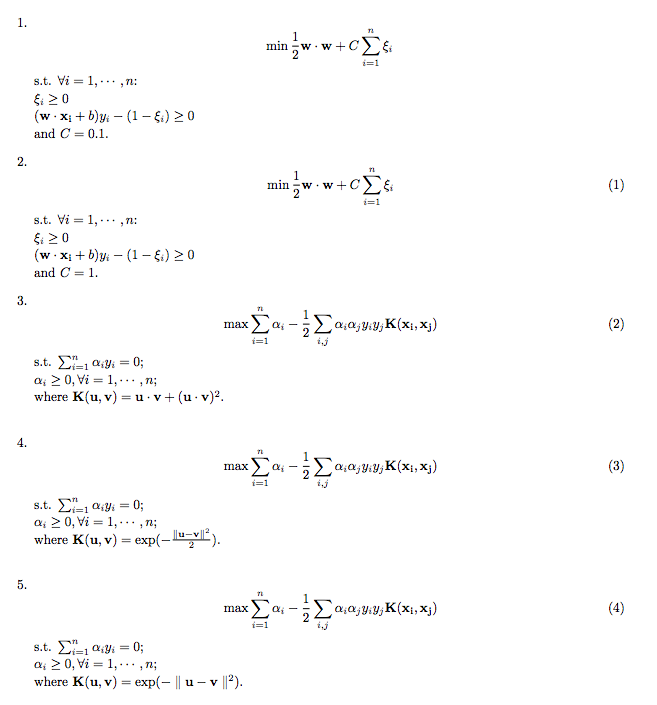
\includegraphics[scale=0.38]{images/svm_equations.png}
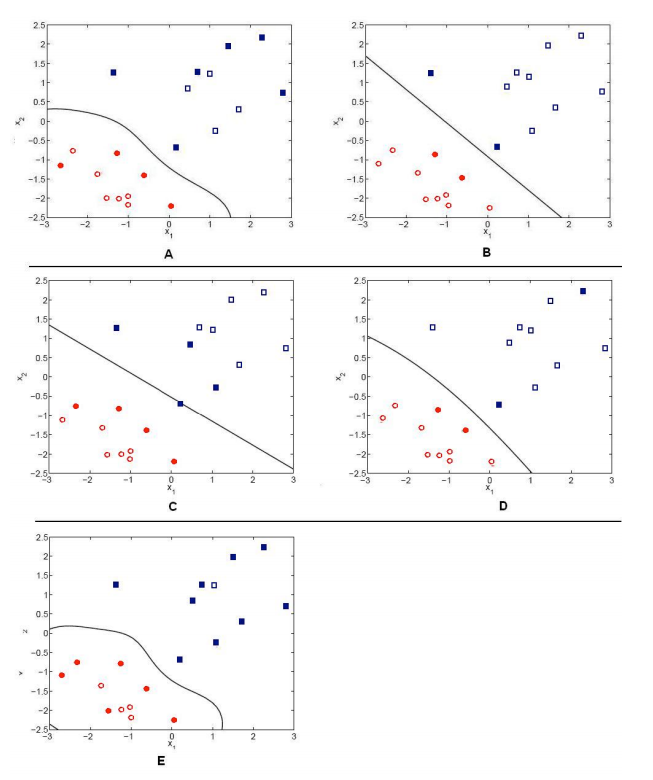
\includegraphics[scale=0.35]{images/svm_plots.png}
\end{center}

\newpage

\subsection*{Задача 4.  Naive Bayes}

С помощью алгоритма Naive Bayes предскажите значение целевой переменной $buy\_computer$ для объекта со следующими значениями признаков:

\begin{verbatim}
age <= 30 & income = medium & student = yes & credit-rating = fair
\end{verbatim}

Для обучения модели используйте данные из таблицы и сглаживане Лапласа.

\begin{center}
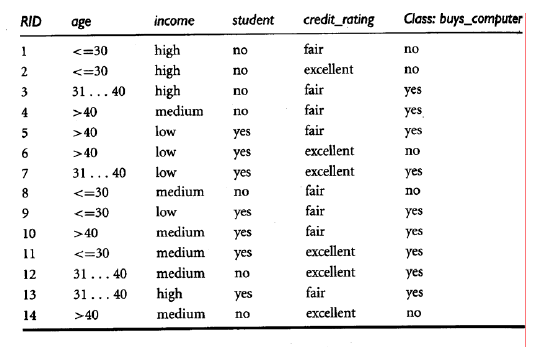
\includegraphics[scale=0.8]{images/nb.png}
\end{center}

\subsection*{Задача 5.  Решающие деревья}

С помощью алгоритма CART постройте первыe два уровня дерева решений на основании представленных данных. Используйте gini impurity.

\begin{center}
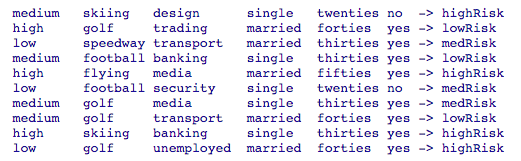
\includegraphics[scale=0.8]{images/dt.png}
\end{center}

\newpage
 
\subsection*{Задача 6.  Bias-Variance tradeoff}

Рассмотрим $N$ пар $(x_i, y_i) \in (\mathcal{X}, \mathcal{Y})$, выбранных независимо в соответствии с распределнием
\[
x_i \sim h(x)
\]
\[
y_i = f(x_i) + \varepsilon_i
\]
\[
\varepsilon_i \sim \mathcal{N}(0, \sigma^2)
\]
Пусть функция, используемая для предсказания, линейна по $y_i$
\[
\hat f(x_0) = \sum_{i=1}^N l_i(x_0, \mathcal{X}) y_i
\] 
Заметим, что веса $l_i(x_0, \mathcal{X})$ не зависят от $y_i$, но зависят от всей выборки $\mathcal{X}$.

\vspace{1em}
\noindent 1. Покажите, что KNN и линейная регрессия являются членами этого семейтсва моделей. Выпишите веса $l_i$ в явном виде.

\noindent 2. Выпишите среднеквадратичную ошибку
\[
E_{\mathcal{Y} | \mathcal{X}} (f(x_0) - \hat f(x_0))^2
\]
в виде суммы variance и квадрата bias.
 
\end{document}